\documentclass{article}
\usepackage{graphicx}
\usepackage{fullpage}
\title{LaTeX Exercise}
\author{Sofie S. Leiszner}
\date{}
\begin{document}
\maketitle

\begin{abstract}
An implementation of the exponential function using LaTeX. 

\end{abstract}

\section{The exponential function}
The exponential function is usually written as a power series~\cite{powerseries}:
	\begin{equation}\label{eq:integ}
\exp x := \sum_{k = 0}^{\infty} \frac{x^k}{k!} = 1 + x + \frac{x^2}{2} + \frac{x^3}{6} + \frac{x^4}{24} + \cdots \;.
    \end{equation}

\section{The quick and dirty implementation - and why it is smart}
A version that is easier to calculate for a computer is the folowing algoritm, which is split into three parts: 
\newline
1) If x is negative, it calculates $1/\exp(-x)$\newline
2) Else if x is larger than 1/8, it calculates $\exp(x/2)^2$ \newline
3) Oterwise if x is positive and larger than 1/8, it uses the Taylor series: 
	\begin{equation}\label{eq:quick}
1+x\cdot(1+x/2\cdot(1+x/3\cdot(1+x/4\cdot(1+x/5\cdot(1+x/6\cdot(1+x/7\cdot(1+x/8\cdot(1+x/9\cdot(1+x/10))))))))) \;.
    \end{equation}
This algoritm is smart compared to the usual sum for computer calculations: 
	\begin{equation}\label{eq:normal}
1+x + x^2/2! + x^3/3! + \cdots \;.
    \end{equation}
For negative x-values, this sum would give alternating positive and negative contributions to the sum, which gives greater uncertainty than the one for the quick-and-dirty algoritm. \newline
The second step ensures, that we only apply the truncanted series to small arguments for which the uncertainty is smaller. \newline
The third step is simply the convulted expression for the Taylor series, which is very accurate for larger positive numbers. It also uses less operations than the sum (if it was also expanded to 10), which used to be a great advantage (slightly smaller advantage now with faster computers though). \newline
 
\section{Figures}
See the figure~(\ref{fig:pyxplot}) on the next page. It plots equation~(\ref{eq:quick}) and the one from the math library.

\begin{figure}
    \centering
    \label{fig:pyxplot}
    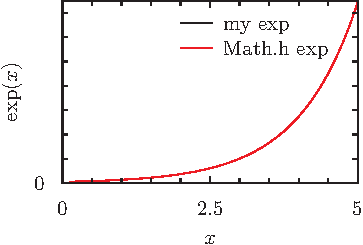
\includegraphics{fig-pyxplot.pdf}
    \caption{The exponential function via pyxplot "pdf" terminal.}
\end{figure}

\begin{thebibliography}{9}
\bibitem{powerseries} Rudin, Walter (1987). Real and complex analysis (3rd ed.). New York: McGraw-Hill. p. 1. ISBN 978-0-07-054234-1.
\end{thebibliography}

\end{document}
